\newpage
\section{The Mezuro Project}
\label{sec:mezuro}
%TODO: The Mezuro Project (5 páginas)

The Mezuro\footnote{\url{http://mezuro.org}} project aims to be an interface which allows, in a flexible way, the extraction, analysis and interpretation of static source code metrics. Licensed under the Affero General Public License version 3 (AGPLv3), it makes the user responsible for defining the metrics she wants to employ on the analysis, keeping track and providing graphical visualization of the evolution of the selected set of metrics. From here the set of selected metrics together with the interpretations for each value  will be referenced just as ``configuration''. Its main academical goals are: to get close to a consensus on which configurations should be employed on the analysis of different kinds of source code written in different programming languages and to search which interpretation should be given to each value obtained for the configuration.

\subsection{Early design}
\label{subsec:early-design}
%% early design (funcionalidades e a forma como foi implementada inicialmente)
%%%% limitations

Initially, we developed a desktop application called Kalibro \cite{de2013kalibro}, written in Java which had many of the features we wanted for source code analysis. At that time, Kalibro already supported the selection and composition of metrics to be employed on the analysis and allowed users to define their own interpretation for the results of each metric calculation. With a created configuration, Kalibro only needed an URL for the source code to start the analysis. The URL could be the path for the source code, compressed in a ZIP or TARBALL file, on the user's computer or the link for the repository where the source code was stored. The source code managers supported included GIT, Subversion, CVS, Mercurial and Bazaar. Finally, the source code could be written in Java, C or C++.

Despite Kalibro being capable to successfully analyze source codes, we could not get close to the consensus we aimed for. The main obstacle was that, with a desktop application, it was not possible to incite the discussion on the configurations employed among developers nor the comparison of results between projects. That was the main reason that motivated the move from a desktop application to a service-based implementation.

\subsection{Service-based implementation}
\label{subsec:service-based-implementation}
%% Services-based implementation
%%%% limitations (Scalability evaluation)

The service-based implementation of the Mezuro project was designed to have a back end, that was a monolithic web service that performed all the database and analysis operations, and a front end, that was a plugin of the Noosfero\footnote{\url{http://noosfero.org/Site}} social network. The first one was described in WSDL and communicated with the front end using SOAP messages. It was still written in Java for it was an extension of Kalibro. As for the back end, we wanted that our users were able to discuss and compare their configuration and results, so a social network seemed a good way to achieve that. We did not want to implement a social network from scratch, though. Noosfero was a good choice for its robust plugin support and for being open source. Our plugin was written in Ruby, using the Ruby on Rails framework. \textbf{Figure \ref{fig:mezuro-noosfero-arch}} represents the state diagram for the service-based implementation. This is a simplified diagram for it omits some entities of our system as the reading groups, which abstract the interpretations given for the metrics and are part of the configurations.

\begin{figure}[htb]
  \centering
  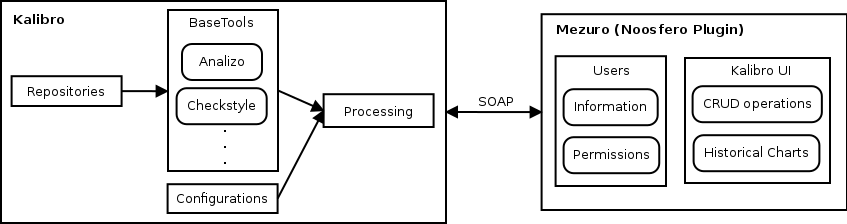
\includegraphics[width=\textwidth]{images/mezuro-noosfero-arch.png}
  \caption{Architecture of the service-based implementation.}
  \label{fig:mezuro-noosfero-arch}
\end{figure}

The main advantage of this implementation was to bring the code analysis tools to the web in a way that multiple users could produce their own configurations, view and share historical results. Unfortunately, we had inconvenient problems. On the front end, the major issue was that the technologies used were outdated making it difficult for maintenance and development. Also, Noosfero had features that we did not need for our social network as the support for communities and events. For the web service being monolithic, minor changes on the source code implied a full deploy of the system and it was hard to understand and modify it. That slowed down our productivity. Still, the main disadvantage was the scalability.

We started worrying about scalability when we were about to release Mezuro to the community. We wanted to assess if Kalibro could keep its performance when changes on the workload occurred. For the tests, we used the Scalability Explorer\cite{moura2013automated} framework. We calculated three metrics available on the framework: speedup, degradation and aggregate performance comparison\cite{li2012catalogue}. Sadly, we found that our most important feature, the process repository operation, was not scalable. Worse, for big workloads Kalibro simply stopped working without errors. Further investigation showed us that this sudden interruption happened due to a deadlock. The problem was on the static thread pool created by Kalibro. By default, Kalibro created a static thread pool with a variable number of threads, depending on the machine it was running on. The threads were kept idle, waiting for some operation to awake them. Each source code analysis required four threads to complete because parts of that operation were made in parallel. The operation awoke the threads on demand, that it, only when it was going to use them. Therefore, if a great number of requests for the process repository operation reached the service simultaneously, those operations would start but would not be able to finish because of a lack of threads available.

With difficulties for modifying the code to support a dynamic thread pool, our solution was to rewrite the service so we could solve the deadlock issue and improve the service architecture.

\subsection{Cloud-based implementation}
\label{subsec:cloud-based-implementation}
%% Cloud-based (explicando que usou micro-services)
%%%% experimental results (mostrar o máximo possível que a coisa funciona e é eficiente, ou seja, atinge os objetivos do artigo).

The rewritten code was split into three different services: Prezento, Kalibro Processor and Kalibro Configurations. The user interface, code analyzer and configuration manager respectively. We designed Kalibro onto two separated services with the intention of leaving each of them with less responsibilities, making them easier to maintain and to extend. Furthermore, it allows other developers to reuse them flexibly. For example, if one desires to implement its own source code analyzer, he can utilize Kalibro Configurations for managing metrics and their interpretations. Those services communicate through HTTP requests encapsulated onto a fourth piece of software called Kalibro Client. All of them are written in Ruby with the support of the Ruby on Rails framework. The reason for switching WSDL and SOAP for RESTful APIs was its significantly simpler implementation.

All this work is based on the micro-service architecture \cite{namiot2014micro}. With this new distributed architecture the platform has more flexibility to scale into the cloud. It, as well, demands less knowledge from developers about the existing code, since they do not need to know all the services but just the one which relates to the feature being implemented and its API. Other advantages are that each service can be written in different programming languages and, for each service runs its own processes, they can be deployed independently. Fault tolerance is also enhanced. The main disadvantages of the micro-services architecture are that it is more complex and, if the API of one of the services change, the others that use it must adapt to keep the communication working.

\textbf{Figure \ref{fig:mezuro-cloud-arch}} refers to the state diagram for the cloud-based implementation. Again, there are implicit details we omitted to keep the simplicity as the Kalibro Client gem that encapsulates the exchanged HTTP messages among the services.

\begin{figure}[htb]
  \centering
  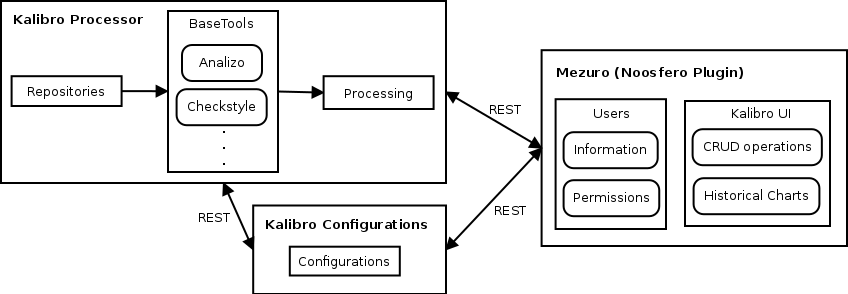
\includegraphics[width=\textwidth]{images/mezuro-cloud-arch.png}
  \caption{Architecture of the cloud-based implementation.}
  \label{fig:mezuro-cloud-arch}
\end{figure}